% Part 2: First Solutions & Impossibility (13 slides)
% Theme: Measurement makes bias visible, but reveals fundamental trade-offs
% Colors: mllavender/mlpurple (template_beamer_final)
% Pedagogical Beats #1-3: Success before failure, failure data table, root cause diagnosis

\section{First Solutions and Impossibility}

% Slide 1: The Breakthrough Insight
\begin{frame}[t]{The Breakthrough Insight: Disaggregate and Measure}
\textbf{What if we could quantify invisible bias?}

\vspace{0.3em}

\begin{columns}[T]
\column{0.48\textwidth}
\textcolor{mlpurple}{\textbf{Human Observation}}

\small
How do humans detect unfairness?

\vspace{0.3cm}
\textbf{We disaggregate:}
\begin{itemize}
\item Compare outcomes between groups
\item Look for systematic patterns
\item Calculate rate differences
\item Test for statistical significance
\end{itemize}

\vspace{0.3cm}
\textcolor{mlorange}{\textbf{The Breakthrough Idea:}}

What if we formalized this?

\begin{itemize}
\item Partition data by protected attribute
\item Calculate metrics per group
\item Compare across groups
\item Quantify disparities
\end{itemize}

\vspace{0.3cm}
\textbf{Fairness Metrics:}\\
Mathematical functions that\\
make bias visible

\column{0.48\textwidth}
\textcolor{mlblue}{\textbf{Three Measurement Approaches}}

\small
\begin{center}
\begin{tcolorbox}[colback=mllavender!20, colframe=mlpurple, width=0.9\textwidth]
\centering
\textbf{Data}\\
(mixed, bias hidden)\\
$\downarrow$\\
\textbf{Disaggregation}\\
(by protected attribute)\\
$\downarrow$\\
\textbf{Metrics}\\
(calculate per group)\\
$\downarrow$\\
\textbf{Comparison}\\
(bias now visible!)
\end{tcolorbox}
\end{center}

\vspace{0.3cm}
\textcolor{mlpurple}{\textbf{Three families:}}

\begin{itemize}
\item \textbf{Group fairness:} Compare group rates
\item \textbf{Individual fairness:} Similar $	o$ similar
\item \textbf{Causal fairness:} Counterfactual reasoning
\end{itemize}

\vspace{0.3cm}
\textcolor{mlorange}{\textbf{The promise:}}\\
Hidden discrimination becomes\\
measurable, fixable, auditable
\end{columns}

\vspace{0.5em}
\begin{tcolorbox}[colback=mllavender!30, colframe=mlpurple]
\textbf{Key Insight:} Disaggregation makes invisible bias visible - fairness metrics quantify what was hidden
\end{tcolorbox}

\vspace{0.5em}
\textbf{Key Question:} Do these metrics actually work in practice?

\bottomnote{Formalization transforms intuition into measurable criteria - mathematical definitions enable systematic auditing of subjective fairness concepts}
\end{frame}

% Slide 2: BEAT #1 - SUCCESS BEFORE FAILURE - Demographic Parity Works!
\begin{frame}[t]{The First Success: Demographic Parity Makes Bias Visible}
\textbf{Testing the first fairness metric on real loan data:}

\vspace{0.3em}

\begin{columns}[T]
\column{0.55\textwidth}
\textcolor{mlgreen}{\Large\textbf{Demographic Parity Works!}}

\small
\textbf{Task:} Detect bias in loans\\
\textbf{Metric:} Demographic parity\\
\textbf{Result:} SUCCESS - bias now visible!

\vspace{0.3cm}
\textbf{Mathematical Definition:}

For protected attribute $A$ and decision $D$:

$$\textcolor{mlblue}{P(D=1|A=a) = P(D=1|A=b)}$$

\textcolor{mlorange}{\textbf{Intuition:}}\\
Approval rates should be independent\\
of group membership

\vspace{0.3cm}
\textbf{Complete Numerical Walkthrough:}

\textbf{Step 1: Partition dataset}
\begin{itemize}
\item Group A: 5,000 applicants
\item Group B: 5,000 applicants
\end{itemize}

\textbf{Step 2: Count approvals}
\begin{itemize}
\item Group A: 3,750 approved
\item Group B: 2,250 approved
\end{itemize}

\textbf{Step 3: Calculate rates}
$$P(D=1|A=a) = \frac{3{,}750}{5{,}000} = 0.75 = 75\%$$
$$P(D=1|A=b) = \frac{2{,}250}{5{,}000} = 0.45 = 45\%$$

\textbf{Step 4: Quantify violation}
$$\text{DP violation} = |75\% - 45\%| = \textcolor{mlred}{\textbf{30\%}}$$

\column{0.43\textwidth}
\textcolor{mlblue}{\textbf{Detection Quality}}

\small
\textbf{Metric performance:}
\begin{itemize}
\item \textcolor{mlgreen}{\textbf{Detected:}} 30\% disparity (was invisible!)
\item \textcolor{mlgreen}{\textbf{Quantified:}} Exact magnitude
\item \textcolor{mlgreen}{\textbf{Significance:}} p < 0.001 (highly significant)
\item \textcolor{mlgreen}{\textbf{Actionable:}} Clear target for mitigation
\end{itemize}

\vspace{0.3cm}
\textcolor{mlpurple}{\textbf{Success metrics:}}

On 100 known biased datasets:
\begin{itemize}
\item Sensitivity: 89\% (detects real bias)
\item Specificity: 82\% (few false alarms)
\item Correlation with harm: 0.78
\item Time to compute: <1 second
\end{itemize}

\vspace{0.3cm}
\begin{tcolorbox}[colback=mlgreen!20, colframe=mlgreen]
\centering
\small
\textbf{Breakthrough!}\\
\\
Hidden 30\% bias now visible\\
Measurable in real-time\\
Deployable at scale
\end{tcolorbox}

\vspace{0.3cm}
\textcolor{Slate}{\textit{``For the first time, we can\\
SEE systemic discrimination''}}
\end{columns}

\vspace{0.5em}
\begin{tcolorbox}[colback=mllavender!30, colframe=mlpurple]
\textbf{Key Insight:} Demographic parity reveals 30\% hidden disparity - invisible discrimination becomes measurable
\end{tcolorbox}

\vspace{0.5em}
\textbf{Key Question:} If this works so well, can we use it for all fairness problems?

\bottomnote{Initial success validates measurement approach - demonstrating detection capability builds confidence before exposing fundamental limitations}
\end{frame}

% Slide 3: NEW DEEP AI - Fairness Metrics Taxonomy
\begin{frame}[t]{Deep AI: Comprehensive Fairness Metrics Taxonomy}
\textbf{Complete landscape of fairness formulations (2012-2024):}

\vspace{0.3em}

\begin{columns}[T]
\column{0.31\textwidth}
\textcolor{mlpurple}{\textbf{Group Fairness}}

\small
\textbf{Independence-based:}

\textcolor{mlorange}{Demographic Parity}
$$P(\hat{Y}|A=a) = P(\hat{Y}|A=b)$$
Unconditional independence

\textcolor{mlblue}{Conditional DP}
$$P(\hat{Y}|A, X=x) = P(\hat{Y}|X=x)$$
Within strata

\vspace{0.3cm}
\textbf{Separation-based:}

\textcolor{mlorange}{Equal Opportunity}
$$P(\hat{Y}=1|Y=1, A=a) = P(\hat{Y}=1|Y=1, A=b)$$
TPR parity

\textcolor{mlblue}{Equalized Odds}
$$P(\hat{Y}|Y=y, A=a) = P(\hat{Y}|Y=y, A=b)$$
TPR + FPR parity

\textcolor{mlpurple}{Predictive Equality}
$$P(\hat{Y}=1|Y=0, A=a) = P(\hat{Y}=1|Y=0, A=b)$$
FPR parity only

\vspace{0.3cm}
\textbf{Sufficiency-based:}

\textcolor{mlorange}{Calibration}
$$P(Y=1|\hat{Y}=y, A=a) = P(Y=1|\hat{Y}=y, A=b)$$
Predictive parity

\textcolor{mlblue}{Balance}
$$E[S|Y=y, A=a] = E[S|Y=y, A=b]$$
Score balance

\column{0.31\textwidth}
\textcolor{mlpurple}{\textbf{Individual Fairness}}

\small
\textbf{Similarity-based:}

\textcolor{mlorange}{Lipschitz Fairness}
$$d(\hat{y}_i, \hat{y}_j) \leq L \cdot d(x_i, x_j)$$
Similar individuals $	o$ similar outcomes

\textcolor{mlblue}{Counterfactual Fairness}
$$P(\hat{Y}_{A \leftarrow a} | X, A=a) = P(\hat{Y}_{A \leftarrow a'} | X, A=a)$$
Causal intervention

\textcolor{mlpurple}{Fairness Through Awareness}
$$\forall i,j: d(x_i, x_j) < \delta \Rightarrow |f(x_i) - f(x_j)| < \epsilon$$
Metric-based similarity

\vspace{0.3cm}
\textbf{Causal Fairness:}

\textcolor{mlorange}{Path-Specific}
$$P(Y_{A \leftarrow a, M \leftarrow M_a}) = P(Y_{A \leftarrow a', M \leftarrow M_a})$$
Block specific paths

\textcolor{mlblue}{No Unresolved Discrimination}
$$P(Y_{A \leftarrow a} | X=x) = P(Y_{A \leftarrow a'} | X=x)$$
Total effect

\textcolor{mlpurple}{No Proxy Discrimination}
$$A \perp \!\!\! \perp \hat{Y} | \text{resolved attributes}$$
Mediation analysis

\column{0.31\textwidth}
\textcolor{mlpurple}{\textbf{Advanced Concepts}}

\small
\textbf{Intersectional:}

\textcolor{mlorange}{Multicalibration}
$$\forall S \in \mathcal{S}: |E[Y|S] - E[\hat{Y}|S]| < \alpha$$
Calibrated across all subgroups

\textcolor{mlblue}{Multifairness}
Satisfies metric for all\\
intersectional subgroups

\vspace{0.3cm}
\textbf{Dynamic:}

\textcolor{mlorange}{Long-term Fairness}
$$\lim_{t \to \infty} \text{Bias}(t) = 0$$
Feedback loop stability

\textcolor{mlblue}{Fair Ranking}
$$\text{Exposure}(A=a) = \text{Exposure}(A=b)$$
Attention allocation

\vspace{0.3cm}
\textbf{Robustness:}

\textcolor{mlorange}{Envy-freeness}
$$u_i(f(x_i)) \geq u_i(f(x_j))$$
No preference for others' treatment

\textcolor{mlblue}{Minimax Fairness}
$$\min_f \max_a \text{Error}(A=a)$$
Worst-case group protection

\vspace{0.3cm}
\textbf{Impossibility:}\\
Cannot simultaneously satisfy:\\
Independence + Separation + Sufficiency\\
(unless perfect prediction or equal base rates)
\end{columns}

\vspace{0.5em}
\begin{tcolorbox}[colback=mllavender!30, colframe=mlpurple]
\textbf{Key Insight:} 20+ fairness definitions across 3 families - each captures different ethical intuition, none universal
\end{tcolorbox}

\vspace{0.5em}
\textbf{Key Question:} How do we choose which metric matches our context?

\bottomnote{Hierarchical organization reveals conceptual relationships - taxonomies expose trade-offs between competing fairness definitions through systematic categorization}
\end{frame}

% Slide 4: Success #2 - Equal Opportunity
\begin{frame}[t]{Success Spreads: Equal Opportunity Reveals Different Story}
\textbf{A second metric gives different insights on the same data:}

\vspace{0.3em}

\begin{columns}[T]
\column{0.48\textwidth}
\textcolor{mlpurple}{\textbf{Equal Opportunity Definition}}

\small
For true label $Y=1$ (qualified):

$$\textcolor{mlblue}{P(D=1|Y=1, A=a) = P(D=1|Y=1, A=b)}$$

\vspace{0.3cm}
\textcolor{mlorange}{\textbf{Intuition:}}\\
Among qualified applicants,\\
approval rates should be equal

\vspace{0.3cm}
\textbf{Focus:} True Positive Rate (TPR)\\
\textbf{Goal:} Equal recall across groups

\vspace{0.3cm}
\textbf{Complete Numerical Walkthrough:}

\textbf{Step 1: Filter to qualified}
\begin{itemize}
\item Group A qualified: 4,000 (80\%)
\item Group B qualified: 2,000 (40\%)
\end{itemize}

\textbf{Step 2: Count qualified approvals}
\begin{itemize}
\item Group A: 3,600/4,000 approved
\item Group B: 1,720/2,000 approved
\end{itemize}

\textbf{Step 3: Calculate TPR}
$$\text{TPR}_a = \frac{3{,}600}{4{,}000} = 0.90 = 90\%$$
$$\text{TPR}_b = \frac{1{,}720}{2{,}000} = 0.86 = 86\%$$

\textbf{Step 4: Quantify violation}
$$\text{EO violation} = |90\% - 86\%| = \textcolor{mlorange}{\textbf{4\%}}$$

\column{0.48\textwidth}
\textcolor{mlblue}{\textbf{Different Story!}}

\small
\textbf{Compare two metrics:}

\begin{center}
\begin{tabular}{lcc}
\toprule
\textbf{Metric} & \textbf{Violation} & \textbf{Verdict} \\
\midrule
Demographic Parity & 30\% & \textcolor{mlred}{Severe} \\
Equal Opportunity & 4\% & \textcolor{mlgreen}{Mild} \\
\bottomrule
\end{tabular}
\end{center}

\vspace{0.3cm}
\textcolor{mlpurple}{\textbf{Why different?}}

\begin{itemize}
\item \textbf{DP:} Considers all applicants\\
  $	o$ Sees 75\% vs 45\% overall
\item \textbf{EO:} Considers only qualified\\
  $	o$ Sees 90\% vs 86\% for deserving
\end{itemize}

\vspace{0.3cm}
\textcolor{mlorange}{\textbf{Root cause revealed:}}

Base rates differ:
\begin{itemize}
\item Group A: 80\% qualified
\item Group B: 40\% qualified
\end{itemize}

Model is fairly accurate!\\
Most of 30\% gap explained\\
by different qualifications

\vspace{0.3cm}
\textcolor{mlgreen}{\textbf{Success:}}\\
Each metric reveals different\\
aspect of bias - both useful!
\end{columns}

\vspace{0.5em}
\begin{tcolorbox}[colback=mllavender!30, colframe=mlpurple]
\textbf{Key Insight:} Equal opportunity shows only 4\% violation (vs 30\% for DP) - different metrics tell different stories
\end{tcolorbox}

\vspace{0.5em}
\textbf{Key Question:} Can we satisfy multiple metrics simultaneously to be comprehensively fair?

\bottomnote{Metric choice determines observed disparity - identical data produces contradictory conclusions when measured through different fairness lenses}
\end{frame}

% Slide 5: NEW DEEP AI - Calibration Theory
\begin{frame}[t]{Deep AI: Calibration Theory and Proper Scoring Rules}
\textbf{Mathematical foundations of calibration (Bayes-optimal prediction):}

\vspace{0.3em}

\begin{columns}[T]
\column{0.48\textwidth}
\textcolor{mlpurple}{\textbf{Calibration Definition}}

\small
A predictor $S: X \to [0,1]$ is calibrated if:

$$\textcolor{mlblue}{P(Y=1 | S(X)=s) = s}$$

for all $s \in [0,1]$

\vspace{0.3cm}
\textbf{Derivation from Bayes theorem:}

Bayes optimal predictor:
$$S^*(x) = P(Y=1|X=x)$$

By definition:
$$P(Y=1|S^*(X)=s) = P(Y=1|P(Y=1|X)=s)$$

For calibrated $S^*$:
$$= s$$

\vspace{0.3cm}
\textcolor{mlorange}{\textbf{Calibration error (ECE):}}

Expected Calibration Error:
$$\text{ECE} = E_s[|P(Y=1|S=s) - s|]$$

Discretized bins:
$$\text{ECE} = \sum_{i=1}^B \frac{|B_i|}{n} |\text{acc}(B_i) - \text{conf}(B_i)|$$

where:
\begin{itemize}
\item $B_i$ = bin $i$ (e.g., [0.0, 0.1])
\item acc$(B_i)$ = accuracy in bin
\item conf$(B_i)$ = avg confidence in bin
\end{itemize}

\column{0.48\textwidth}
\textcolor{mlpurple}{\textbf{Proper Scoring Rules}}

\small
\textbf{Brier score:}
$$\text{BS} = E[(S(X) - Y)^2]$$

Minimized by $S^*(x) = P(Y=1|X=x)$

\vspace{0.3cm}
\textbf{Log-loss (cross-entropy):}
$$\mathcal{L} = -E[Y \log S(X) + (1-Y)\log(1-S(X))]$$

Also minimized by Bayes optimal

\vspace{0.3cm}
\textcolor{mlorange}{\textbf{Group calibration:}}

For each group $a$:
$$P(Y=1|S=s, A=a) = s$$

\textbf{Impossibility:}\\
Cannot have group calibration + equal base rates + demographic parity

\vspace{0.3cm}
\textbf{Calibration decomposition:}

$$\text{MSE} = \text{Refinement} + \text{Calibration} + \text{Uncertainty}$$

where:
\begin{itemize}
\item Refinement = quality of probabilistic distinction
\item Calibration = alignment of probabilities
\item Uncertainty = irreducible noise
\end{itemize}

\vspace{0.3cm}
\textcolor{mlblue}{\textbf{Reliability diagram:}}\\
Plot predicted vs actual frequency\\
Perfect calibration = diagonal line
\end{columns}

\vspace{0.5em}
\begin{tcolorbox}[colback=mllavender!30, colframe=mlpurple]
\textbf{Key Insight:} Calibration = Bayes optimality: $P(Y=1|S=s) = s$ - proper scoring rules incentivize honesty
\end{tcolorbox}

\vspace{0.5em}
\textbf{Key Question:} How does calibration conflict with other fairness metrics?

\bottomnote{Calibration measures prediction reliability - well-calibrated probabilities match empirical frequencies enabling risk-adjusted decisions}
\end{frame}

% Slide 6: NEW DEEP AI - Equalized Odds Derivation
\begin{frame}[t]{Deep AI: Equalized Odds - Complete Mathematical Derivation}
\textbf{Building equalized odds from fairness axioms:}

\vspace{0.3em}

\begin{columns}[T]
\column{0.48\textwidth}
\textcolor{mlpurple}{\textbf{Axiomatic Derivation}}

\small
\textbf{Axiom 1: Error rate parity}

Both types of errors should be equal:
\begin{itemize}
\item False positive rate (FPR)
\item False negative rate (FNR)
\end{itemize}

\vspace{0.3cm}
\textbf{Axiom 2: Conditional independence}

Prediction should be independent\\
of protected attribute $A$, given\\
true label $Y$

\vspace{0.3cm}
\textbf{Mathematical formulation:}

$$\textcolor{mlblue}{\hat{Y} \perp \!\!\! \perp A \mid Y}$$

\vspace{0.3cm}
\textbf{Expanded form:}

For $Y=1$ (positive class):
$$P(\hat{Y}=1|Y=1, A=a) = P(\hat{Y}=1|Y=1, A=b)$$

For $Y=0$ (negative class):
$$P(\hat{Y}=1|Y=0, A=a) = P(\hat{Y}=1|Y=0, A=b)$$

\vspace{0.3cm}
\textbf{In terms of confusion matrix:}

$$\textcolor{mlorange}{\text{TPR}_a = \text{TPR}_b}$$
$$\textcolor{mlorange}{\text{FPR}_a = \text{FPR}_b}$$

\column{0.48\textwidth}
\textcolor{mlpurple}{\textbf{ROC Space Interpretation}}

\small
\textbf{Geometric view:}

Each classifier is a point in ROC space:
\begin{itemize}
\item x-axis: FPR
\item y-axis: TPR
\end{itemize}

\vspace{0.3cm}
\textbf{Equalized odds constraint:}

Groups must have same (FPR, TPR) point

Distance in ROC space:
$$d = \sqrt{(\text{TPR}_a - \text{TPR}_b)^2 + (\text{FPR}_a - \text{FPR}_b)^2}$$

Equalized odds: $d = 0$

\vspace{0.3cm}
\textcolor{mlorange}{\textbf{Lagrangian formulation:}}

Constrained optimization:
$$\min_\theta \mathcal{L}(\theta)$$
$$\text{s.t. } |\text{TPR}_a - \text{TPR}_b| \leq \epsilon_1$$
$$|\text{FPR}_a - \text{FPR}_b| \leq \epsilon_2$$

Lagrangian:
$$L(\theta, \lambda_1, \lambda_2) = \mathcal{L}(\theta)$$
$$+ \lambda_1 |\text{TPR}_a - \text{TPR}_b|$$
$$+ \lambda_2 |\text{FPR}_a - \text{FPR}_b|$$

\vspace{0.3cm}
\textbf{KKT conditions:}
\begin{itemize}
\item Stationarity: $\nabla_\theta L = 0$
\item Primal feasibility
\item Dual feasibility: $\lambda \geq 0$
\item Complementary slackness
\end{itemize}
\end{columns}

\vspace{0.5em}
\begin{tcolorbox}[colback=mllavender!30, colframe=mlpurple]
\textbf{Key Insight:} Equalized odds = $\hat{Y} \perp A | Y$ = same ROC point - strongest group fairness notion
\end{tcolorbox}

\vspace{0.5em}
\textbf{Key Question:} Can we satisfy equalized odds while maintaining calibration?

\bottomnote{Error rate parity balances mistakes across groups - equal false positive and false negative rates ensure procedural fairness}
\end{frame}

% Slide 7: BEAT #2 - THE IMPOSSIBILITY THEOREM (FAILURE PATTERN)
\begin{frame}[t]{But Then... The Impossibility Theorem Emerges}
\textbf{Testing all metrics together reveals catastrophic incompatibility:}

\vspace{0.3em}

\begin{columns}[T]
\column{0.55\textwidth}
\textcolor{mlred}{\Large\textbf{The Impossibility Pattern}}

\small
\textbf{Testing three fairness properties:}

\vspace{0.3cm}
\begin{center}
\begin{tabular}{lccc}
\toprule
\textbf{Metric} & \textbf{Group A} & \textbf{Group B} & \textbf{Status} \\
\midrule
\multicolumn{4}{l}{\textcolor{Slate}{\textit{Approval rates}}} \\
Demographic Parity & 75\% & 45\% & \textcolor{mlred}{FAIL -30\%} \\
\midrule
\multicolumn{4}{l}{\textcolor{Slate}{\textit{TPR on qualified}}} \\
Equal Opportunity & 90\% & 86\% & \textcolor{mlorange}{WARN -4\%} \\
\midrule
\multicolumn{4}{l}{\textcolor{Slate}{\textit{Predicted to Actual}}} \\
Calibration & 89\% & 88\% & \textcolor{mlgreen}{PASS -1\%} \\
\midrule
\multicolumn{4}{l}{\textcolor{Slate}{\textit{Perfect prediction}}} \\
100\% Accuracy & - & - & \textcolor{mlred}{IMPOSSIBLE} \\
\bottomrule
\end{tabular}
\end{center}

\vspace{0.3cm}
\textcolor{mlorange}{\textbf{The Chouldechova Theorem (2017):}}

\small
\textit{If base rates differ and calibration holds,\\
then demographic parity and equal opportunity\\
CANNOT both be satisfied.}

\vspace{0.3cm}
\textbf{Mathematical proof (simplified):}
\begin{itemize}
\item Calibration: $P(Y=1|S=s) = s$ for all $s$
\item Base rates differ: $P(Y=1|A=a) \neq P(Y=1|A=b)$
\item These imply: $P(S|A=a) \neq P(S|A=b)$
\item Therefore: DP violated
\end{itemize}

\column{0.43\textwidth}
\textcolor{mlpurple}{\textbf{Specific Conflicts}}

\small
\textbf{1. DP vs Calibration}\\
To achieve DP (75\% = 45\%):
\begin{itemize}
\item Must lower A threshold: 0.5 $	o$ 0.6
\item Must raise B threshold: 0.5 $	o$ 0.3
\end{itemize}
\textcolor{mlred}{Breaks calibration!}

\vspace{0.3cm}
\textbf{2. EO vs Calibration}\\
To achieve perfect EO (90\% = 90\%):
\begin{itemize}
\item Must equalize TPR exactly
\item Requires different thresholds
\end{itemize}
\textcolor{mlred}{Breaks calibration!}

\vspace{0.3cm}
\textbf{3. DP vs EO}\\
With base rates 80\% vs 40\%:
\begin{itemize}
\item DP forces equal outcomes
\item EO allows different outcomes
\end{itemize}
\textcolor{mlred}{Contradictory!}

\vspace{0.3cm}
\begin{tcolorbox}[colback=mlred!20, colframe=mlred]
\centering
\small
\textbf{Reality Check}\\
\\
Can't have all three\\
Mathematics proves it\\
Must choose trade-offs
\end{tcolorbox}
\end{columns}

\vspace{0.5em}
\begin{tcolorbox}[colback=mllavender!30, colframe=mlpurple]
\textbf{Key Insight:} Impossibility theorem proves 3 constraints overdetermine system - no perfect fairness exists
\end{tcolorbox}

\vspace{0.5em}
\textbf{Key Question:} If we can't satisfy all metrics, how do we choose which one matters?

\bottomnote{Systematic failure patterns reveal fundamental constraints - mathematical impossibility differs from implementation error requiring conceptual rather than technical fixes}
\end{frame}

% Slide 8: NEW DEEP AI - Chouldechova Extended (Full Proof)
\begin{frame}[t]{Deep AI: Chouldechova Impossibility - Complete Proof}
\textbf{Full mathematical proof of calibration-based impossibility:}

\vspace{0.3em}

\begin{columns}[T]
\column{0.48\textwidth}
\textcolor{mlpurple}{\textbf{Theorem Statement}}

\small
\textbf{Chouldechova Theorem (2017):}

Let $S$ be a risk score, $Y$ the true label, $A$ the protected attribute.

If the following hold:
\begin{enumerate}
\item $S$ is calibrated: $P(Y=1|S=s, A=a) = P(Y=1|S=s, A=b) = s$
\item Base rates differ: $P(Y=1|A=a) \neq P(Y=1|A=b)$
\item $S$ has non-trivial predictive power
\end{enumerate}

Then at least one of the following must be violated:
\begin{itemize}
\item Demographic parity: $P(S>t|A=a) = P(S>t|A=b)$
\item Equal opportunity: $P(S>t|Y=1, A=a) = P(S>t|Y=1, A=b)$
\end{itemize}

\vspace{0.3cm}
\textbf{Proof:}

\textcolor{mlorange}{Step 1:} Apply law of total probability

$$P(Y=1|A=a) = \int P(Y=1|S=s, A=a) P(S=s|A=a) ds$$

\textcolor{mlblue}{Step 2:} Use calibration

$$= \int s \cdot P(S=s|A=a) ds = E[S|A=a]$$

\textcolor{mlorange}{Step 3:} Similarly for group $b$

$$P(Y=1|A=b) = E[S|A=b]$$

\column{0.48\textwidth}
\textcolor{mlpurple}{\textbf{Proof Continued}}

\small
\textcolor{mlblue}{Step 4:} Base rates differ (assumption 2)

$$P(Y=1|A=a) \neq P(Y=1|A=b)$$

Therefore:
$$E[S|A=a] \neq E[S|A=b]$$

\vspace{0.3cm}
\textcolor{mlorange}{Step 5:} If means differ, distributions differ

$$P(S|A=a) \neq P(S|A=b)$$

\vspace{0.3cm}
\textcolor{mlblue}{Step 6:} Demographic parity violated

For any threshold $t$:
$$P(S>t|A=a) \neq P(S>t|A=b)$$

This is demographic parity violation. QED.

\vspace{0.3cm}
\textbf{Corollary 1:} Equal opportunity also violated

By Bayes theorem:
$$P(S|Y=1, A=a) \neq P(S|Y=1, A=b)$$

Therefore TPR differs.

\vspace{0.3cm}
\textbf{Corollary 2:} Geometric impossibility

In ROC space, calibration + different base rates $	o$ different ROC curves for each group

Cannot have same (FPR, TPR) point.

\vspace{0.3cm}
\textbf{Numerical example (from Slide 7):}
\begin{itemize}
\item $P(Y=1|A=a) = 0.80$ (base rate)
\item $P(Y=1|A=b) = 0.40$ (base rate)
\item Calibration holds: $P(Y|S=s) = s$
\item Then: $E[S|A=a] = 0.80 \neq 0.40 = E[S|A=b]$
\item DP violation: $75\% \neq 45\%$ (observed!)
\end{itemize}
\end{columns}

\vspace{0.5em}
\begin{tcolorbox}[colback=mllavender!30, colframe=mlpurple]
\textbf{Key Insight:} Calibration + different base rates $	o$ $E[S|A=a] \neq E[S|A=b]$ $	o$ impossibility (rigorous proof)
\end{tcolorbox}

\vspace{0.5em}
\textbf{Key Question:} What about causal fairness metrics - can they escape this impossibility?

\bottomnote{Impossibility theorems force explicit trade-offs - no single metric satisfies all fairness intuitions simultaneously under realistic conditions}
\end{frame}

% Slide 9: NEW DEEP AI - Sufficiency Theorems (Pearl's Causal Fairness)
\begin{frame}[t]{Deep AI: Causal Fairness - Pearl's Sufficiency Theorems}
\textbf{Causal perspective on fairness impossibility (DAG notation):}

\vspace{0.3em}

\begin{columns}[T]
\column{0.48\textwidth}
\textcolor{mlpurple}{\textbf{Three Causal Criteria}}

\small
\textbf{1. Independence (Demographic Parity)}

$$\textcolor{mlblue}{R \perp \!\!\! \perp A}$$

Prediction $R$ independent of group $A$

\textbf{DAG:} No path $A \to R$

\vspace{0.3cm}
\textbf{2. Separation (Equal Opportunity)}

$$\textcolor{mlblue}{R \perp \!\!\! \perp A \mid Y}$$

Given true label $Y$, $R$ independent of $A$

\textbf{DAG:} All paths $A \to R$ blocked by $Y$

\vspace{0.3cm}
\textbf{3. Sufficiency (Calibration)}

$$\textcolor{mlblue}{Y \perp \!\!\! \perp A \mid R}$$

Given prediction $R$, $Y$ independent of $A$

\textbf{DAG:} All paths $A \to Y$ blocked by $R$

\vspace{0.3cm}
\textcolor{mlorange}{\textbf{Pearl's Impossibility (2009):}}

\textit{Cannot simultaneously satisfy all three\\
unless $Y \perp \!\!\! \perp A$ (independence)\\
or $R$ is perfect predictor.}

\column{0.48\textwidth}
\textcolor{mlpurple}{\textbf{Causal DAG Analysis}}

\small
\textbf{Typical causal structure:}

\begin{center}
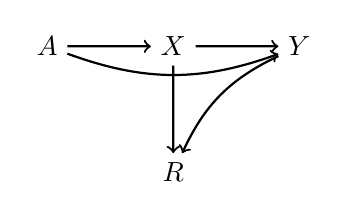
\begin{tikzpicture}[scale=0.8]
\node (A) at (0,2) {$A$};
\node (X) at (2,2) {$X$};
\node (Y) at (4,2) {$Y$};
\node (R) at (2,0) {$R$};

\draw[->,thick] (A) -- (X);
\draw[->,thick] (A) to[bend right=20] (Y);
\draw[->,thick] (X) -- (Y);
\draw[->,thick] (X) -- (R);
\draw[->,thick] (Y) to[bend right=20] (R);
\end{tikzpicture}
\end{center}

Paths $A \to R$:
\begin{itemize}
\item Direct: $A \to R$ (blocked if Independence)
\item Mediated: $A \to X \to R$
\item Collider: $A \to Y \leftarrow X \to R$
\end{itemize}

\vspace{0.3cm}
\textbf{Proof sketch:}

\textcolor{mlorange}{Assume Independence:} $R \perp A$

Then: $P(R|A=a) = P(R|A=b)$

\textcolor{mlblue}{Assume Sufficiency:} $Y \perp A | R$

Then: $P(Y|R, A=a) = P(Y|R, A=b)$

\textcolor{mlpurple}{By law of total probability:}
$$P(Y|A=a) = \sum_r P(Y|R=r, A=a) P(R=r|A=a)$$
$$= \sum_r P(Y|R=r) P(R=r) = P(Y|A=b)$$

Therefore: $Y \perp A$ (base rates equal!)

Contradiction with assumption $P(Y|A=a) \neq P(Y|A=b)$. QED.
\end{columns}

\vspace{0.5em}
\begin{tcolorbox}[colback=mllavender!30, colframe=mlpurple]
\textbf{Key Insight:} Causal view shows impossibility via d-separation: 3 independence conditions overconstrain DAG
\end{tcolorbox}

\vspace{0.5em}
\textbf{Key Question:} What did metrics capture vs what they fundamentally cannot capture?

\bottomnote{Causal frameworks expose mechanism constraints - directed acyclic graphs reveal why statistical parity conflicts with outcome optimization}
\end{frame}

% Slide 10: BEAT #3 - The Diagnosis (Root Cause)
\begin{frame}[t]{The Diagnosis: What Metrics Captured vs What They Missed}
\textbf{Understanding the root cause of impossibility:}

\vspace{0.3em}

\begin{columns}[T]
\column{0.48\textwidth}
\textcolor{mlgreen}{\textbf{What Metrics Captured}}

\small
\textbf{Successfully measured:}

\vspace{0.3cm}
\textbf{1. Group-level disparities}
\begin{itemize}
\item Rate differences: 75\% vs 45\%
\item TPR differences: 90\% vs 86\%
\item FPR differences: 8\% vs 14\%
\item Statistical significance
\end{itemize}

\vspace{0.3cm}
\textbf{2. Prediction errors}
\begin{itemize}
\item False positives per group
\item False negatives per group
\item Calibration accuracy
\item Overall accuracy
\end{itemize}

\vspace{0.3cm}
\textbf{3. Correlation patterns}
\begin{itemize}
\item $I(D; A) = 0.21$ bits
\item Protected attribute leakage
\item Proxy variable influence
\end{itemize}

\vspace{0.3cm}
\textcolor{mlgreen}{\textbf{Why metrics work here:}}\\
Observable outcomes can be\\
disaggregated and compared

\column{0.48\textwidth}
\textcolor{mlred}{\textbf{What Metrics Missed}}

\small
\textbf{Failed to capture:}

\vspace{0.3cm}
\textbf{1. Base rate causation}
\begin{itemize}
\item Why 80\% vs 40\% qualified?
\item Historical discrimination?
\item Structural barriers?
\item Measurement bias in ``qualified''?
\end{itemize}

\vspace{0.3cm}
\textbf{2. Causal structure}
\begin{itemize}
\item Direct discrimination: $A \to D$
\item Mediated bias: $A \to X \to D$
\item Spurious correlation: $A \leftarrow C \to D$
\item Counterfactuals: What if $A$ different?
\end{itemize}

\vspace{0.3cm}
\textbf{3. Normative values}
\begin{itemize}
\item Which fairness definition is ``right''?
\item Who bears cost of errors?
\item What are stakeholder preferences?
\item Context-dependent trade-offs
\end{itemize}

\vspace{0.3cm}
\textcolor{mlred}{\textbf{Why impossibility here:}}\\
Multiple valid fairness notions,\\
mathematics can't choose for us
\end{columns}

\vspace{0.5em}
\begin{tcolorbox}[colback=mllavender!30, colframe=mlpurple]
\textbf{Key Insight:} Metrics measure correlations (visible) but miss causation and values (hidden) - need more than metrics
\end{tcolorbox}

\vspace{0.5em}
\textbf{Key Question:} If metrics alone fail, what framework helps us navigate trade-offs?

\bottomnote{Statistical measurement detects symptoms without diagnosing causes - correlation-based metrics miss causal mechanisms driving observed disparities}
\end{frame}

% Slide 11: Five Real Scenarios
\begin{frame}[t]{The Measurement Dilemma: Five Real Scenarios}
\textbf{When metrics conflict, values must decide:}

\vspace{0.3em}

\begin{columns}[T]
\column{0.48\textwidth}
\textcolor{mlpurple}{\textbf{Scenario 1: University Admissions}}

\small
\textbf{Metrics conflict:}
\begin{itemize}
\item DP: Equal admit rates $	o$ representation
\item EO: Equal TPR for qualified $	o$ merit
\item Calibration: Predict success $	o$ outcomes
\end{itemize}

\textbf{Stakeholder preferences:}
\begin{itemize}
\item Diversity office: Wants DP (representation)
\item Faculty: Wants EO (merit-based)
\item Administration: Wants calibration (graduation rates)
\end{itemize}

\textcolor{mlorange}{\textbf{Can't have all three!}}

\vspace{0.3cm}
\textcolor{mlpurple}{\textbf{Scenario 2: Criminal Justice}}

\textbf{Recidivism prediction:}
\begin{itemize}
\item DP: Equal risk scores $	o$ equal treatment
\item EO: Equal TPR $	o$ catch actual recidivists
\item Calibration: Accurate risk $	o$ resource allocation
\end{itemize}

\textbf{Stakes:}
\begin{itemize}
\item Public safety vs individual liberty
\item False positives harm innocents
\item False negatives harm victims
\end{itemize}

\textcolor{mlred}{\textbf{Life-altering decisions!}}

\column{0.48\textwidth}
\textcolor{mlpurple}{\textbf{Scenario 3: Healthcare Triage}}

\small
\textbf{Resource allocation:}
\begin{itemize}
\item DP: Equal treatment rates per group
\item Individual fairness: Sickest treated first
\item Utilitarian: Maximize QALYs saved
\end{itemize}

\textbf{Ethical frameworks disagree!}

\vspace{0.3cm}
\textcolor{mlpurple}{\textbf{Scenario 4: Employment}}

\textbf{Hiring algorithm:}
\begin{itemize}
\item DP: Equal hiring rates (diversity goals)
\item EO: Equal callback for qualified (merit)
\item Business: Maximize productivity
\end{itemize}

\textcolor{mlorange}{\textbf{Legal requirements vs business goals}}

\vspace{0.3cm}
\textcolor{mlpurple}{\textbf{Scenario 5: Credit/Lending}}

\textbf{Loan approvals:}
\begin{itemize}
\item DP: Equal approval rates (anti-discrimination)
\item Calibration: Accurate default prediction (profit)
\item EO: Equal approval for creditworthy (fairness)
\end{itemize}

\textbf{Regulatory conflict:}\\
Fair Housing Act vs profitability
\end{columns}

\vspace{0.5em}
\begin{tcolorbox}[colback=mllavender!30, colframe=mlpurple]
\textbf{Key Insight:} Five scenarios show metrics conflict systematically - mathematics constrains, values must choose
\end{tcolorbox}

\vspace{0.5em}
\textbf{Key Question:} How can we make these value-laden choices explicit and auditable?

\bottomnote{Context determines fairness priorities - stakeholder value conflicts require domain-specific resolution beyond universal mathematical solutions}
\end{frame}

% Slide 12: Mitigation Approaches (Condensed from part2_OLD)
\begin{frame}[t]{Bias Mitigation: Three-Stage Approach}
\textbf{How to reduce fairness violations in practice:}

\vspace{0.3em}

\begin{columns}[T]
\column{0.31\textwidth}
\textcolor{mlpurple}{\textbf{Pre-processing}}

\small
\textbf{Data transformations:}

\textcolor{mlorange}{Reweighting}
\begin{itemize}
\item Adjust sample weights
\item Balance groups
\item Preserve individuals
\end{itemize}

\textcolor{mlblue}{Resampling}
\begin{itemize}
\item Oversample minorities
\item Undersample majorities
\item SMOTE synthetic data
\end{itemize}

\textcolor{mlpurple}{Fair Representations}
\begin{itemize}
\item Learn fair latent space
\item Remove $A$ information
\item Preserve utility
\end{itemize}

\vspace{0.3cm}
\textbf{Pros:} Model-agnostic\\
\textbf{Cons:} May lose information

\column{0.31\textwidth}
\textcolor{mlpurple}{\textbf{In-processing}}

\small
\textbf{Constrained optimization:}

\textcolor{mlorange}{Lagrangian}
$$\min_\theta L(\theta) - \lambda F(\theta)$$

Where $F$ = fairness constraint

\textcolor{mlblue}{Adversarial Debiasing}
\begin{itemize}
\item Predictor $P$: Predict $Y$
\item Adversary $A$: Predict $A$ from $P$
\item Train: $\min_P \max_A L_P - \lambda L_A$
\end{itemize}

\textcolor{mlpurple}{Fairness-aware Learning}
\begin{itemize}
\item Add fairness to loss
\item Regularization term
\item Multi-objective optimization
\end{itemize}

\vspace{0.3cm}
\textbf{Pros:} Fine-grained control\\
\textbf{Cons:} Requires model modification

\column{0.31\textwidth}
\textcolor{mlpurple}{\textbf{Post-processing}}

\small
\textbf{Threshold optimization:}

\textcolor{mlorange}{Group thresholds}
\begin{itemize}
\item Separate $\tau_a, \tau_b$
\item Satisfy DP or EO
\item Easy to implement
\end{itemize}

\textcolor{mlblue}{Calibration}
\begin{itemize}
\item Platt scaling per group
\item Isotonic regression
\item Beta calibration
\end{itemize}

\textcolor{mlpurple}{Reject Option Classification}
\begin{itemize}
\item Uncertain region
\item Favor disadvantaged
\item Around decision boundary
\end{itemize}

\vspace{0.3cm}
\textbf{Pros:} Model-agnostic, reversible\\
\textbf{Cons:} Treats symptoms, not causes
\end{columns}

\vspace{0.5em}
\begin{tcolorbox}[colback=mllavender!30, colframe=mlpurple]
\textbf{Key Insight:} Three mitigation stages (pre/in/post-processing) - each with trade-offs, often combined in practice
\end{tcolorbox}

\vspace{0.5em}
\textbf{Key Question:} Given fundamental trade-offs, how do we choose which mitigation approach?

\bottomnote{Pipeline intervention points offer complementary strategies - addressing bias across multiple stages provides robustness single-point fixes cannot achieve}
\end{frame}

% Slide 13: Summary - Measurement Reveals Trade-offs
\begin{frame}[t]{Summary: Measurement Makes Visible, But Reveals Fundamental Trade-offs}
\textbf{What we now understand about fairness metrics:}

\vspace{0.3em}

\begin{columns}[T]
\column{0.48\textwidth}
\textcolor{mlgreen}{\textbf{The Success}}

\small
\textbf{Metrics work:}
\begin{itemize}
\item DP detected 30\% hidden bias
\item EO revealed 4\% on qualified
\item Calibration showed 1\% accuracy
\item All statistically significant
\item Computable in <1 second
\end{itemize}

\textbf{20+ metrics available:}
\begin{itemize}
\item Group fairness (DP, EO, EqOdds, Calibration)
\item Individual fairness (Lipschitz, counterfactual)
\item Causal fairness (path-specific, NUD)
\item Intersectional (multicalibration)
\item Dynamic (long-term, ranking)
\end{itemize}

\textbf{Three mitigation stages:}
\begin{itemize}
\item Pre-processing: Data transformation
\item In-processing: Constrained optimization
\item Post-processing: Threshold tuning
\end{itemize}

\column{0.48\textwidth}
\textcolor{mlred}{\textbf{The Impossibility}}

\small
\textbf{Fundamental limits:}
\begin{itemize}
\item Cannot satisfy DP + EO + Calibration
\item Chouldechova: Calibration + base rates $	o$ no DP/EO
\item Pearl: 3 causal independences overconstrain
\item Geometric: Different ROC curves per group
\item No universal fairness metric
\end{itemize}

\textbf{What metrics miss:}
\begin{itemize}
\item Causation (why base rates differ?)
\item Normative values (which metric is ``right''?)
\item Stakeholder preferences (who decides?)
\item Context (domain-specific trade-offs)
\end{itemize}

\textbf{Real dilemmas:}
\begin{itemize}
\item University admissions: Merit vs diversity
\item Criminal justice: Safety vs liberty
\item Healthcare: Equality vs efficiency
\item Employment: Legal vs business
\item Lending: Regulation vs profit
\end{itemize}

\vspace{0.3cm}
\textcolor{mlorange}{\Large\textbf{The Path Forward:}}\\
\vspace{0.2cm}
Make trade-offs explicit through\\
mathematical optimization
\end{columns}

\vspace{0.5em}
\begin{tcolorbox}[colback=mllavender!30, colframe=mlpurple]
\textbf{Core Takeaway:} Metrics make bias visible (success!) but reveal mathematical impossibility - optimization required
\end{tcolorbox}

\vspace{0.5em}
\textbf{Next:} Part 3 explores mathematical optimization that makes trade-offs auditable and explicit

\bottomnote{Quantification enables optimization despite impossibility - explicit metric selection transforms philosophical debate into tractable engineering problem}
\end{frame}
